\begin{frame}{recall: data/instruction memory}
    \begin{itemize}
    \item model in CPU: one cycle per access
    \vspace{.5cm}
    \item but earlier --- had to talk to memory on different chip
    \item can't do that in one cycle
    \vspace{.5cm}
    \item solution: keep copies of part of memory (``cache'')
        \begin{itemize}
        \item copy can be accessed quickly
        \item hope: almost always use copy?
        \end{itemize}
    \end{itemize}
\end{frame}

\usetikzlibrary{arrows.meta,calc,patterns,positioning}
\begin{frame}{2004 CPU}
    \begin{tikzpicture}[scale=1.25]
\clip (1,0) rectangle (14, 7);
\node[anchor=south west] (diePhoto) at (0,0) {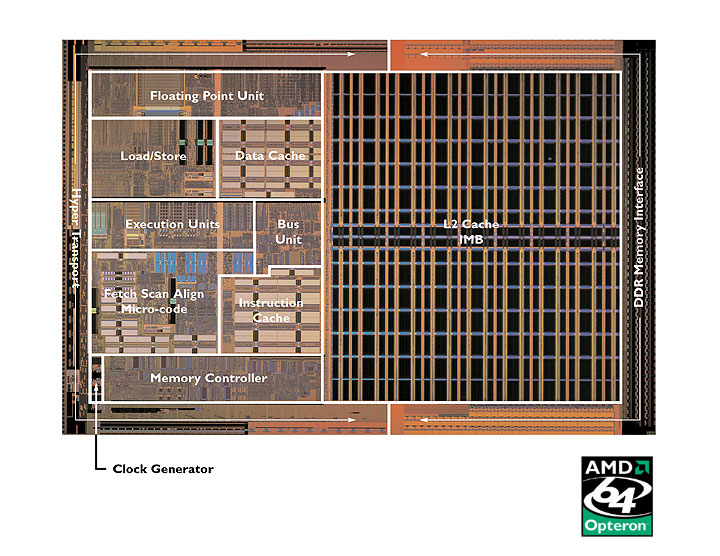
\includegraphics[width=11.25cm]{../caching/Opteron_die_labelled.jpg}};
%\draw[red] (0, 0) grid (9,7);
    \newcommand{\pyrShift}{0.5cm}
\onslide<2->{
    \draw[fill=red,opacity=0.6] (1.9,6.2) rectangle (2.4,5.8);
    \draw[fill=red,opacity=0.6] (1.7,4.2) rectangle (1.9,4.6);

    \begin{scope}[xshift=\pyrShift]
    \draw[fill=red!60!white] (10,7) -- (9.75,6.5) -- (10.25,6.5) -- cycle;
    \node[anchor=west] at (10.1, 6.75) {Registers};
    \end{scope}
}
\onslide<3->{
    %\draw[fill=orange,opacity=0.6] (2.95,2.7) rectangle (4.2,3.6);
    \draw[fill=orange,opacity=0.6] (2.95,2.7) -| (4.2,3.8) -| (3.6,3.65) -- (2.95,3.65) -- (2.95,2.7);
    \draw[fill=orange,opacity=0.6] (2.95,4.6) rectangle (4.2,5.6);

    \begin{scope}[xshift=\pyrShift]
    \draw[fill=orange!60!white] (9.5,6) -- (9.75,6.5) -- (10.25,6.5) -- (10.5,6) -- cycle;
    \node[anchor=west] at (10.35,6.25) {L1 cache};
    \end{scope}
}
\onslide<4->{
    \draw[fill=yellow,opacity=0.6] (4.2,2.1) rectangle (7.9,6.25);
    
    \begin{scope}[xshift=\pyrShift]
    \draw[fill=yellow!60!white] (9.25,5.5) -- (9.5,6) -- (10.5,6) -- (10.75,5.5) -- cycle;
    \node[anchor=west] at (10.6,5.75) {L2 cache};
    \end{scope}
}
\onslide<6->{
    \begin{scope}[xshift=\pyrShift]
    \draw[pattern color=green!60!white,pattern=north west lines] (9.0,5.) -- (9.25,5.5) -- (10.75,5.5) -- (11.,5.) -- cycle;
    \node[anchor=west] at (10.85,5.25) {L3 cache};
    \draw[fill=blue!60!white] (8.5,4.) -- (9.,5.) -- (11,5.) -- (11.5,4.) -- cycle;
    \node[anchor=center,align=center] at (10.,4.5) {main\\memory};
    \end{scope}
}
\onslide<7->{
    \begin{scope}[xshift=\pyrShift]
    \fill[white,opacity=0.9] (7.0,4.5) rectangle (8.4,10.0);
    \begin{scope}[font=\fontsize{10}{11}\selectfont]
        \node[anchor=east] at (9.,6.75) {$<1$ ns};
        \node[anchor=east] at (9.,6.25) {$\sim1$ ns};
        \node[anchor=east] at (9.,5.75) {$\sim5$ ns};
        \node[anchor=east] at (9.,5.25) {$\sim20$ ns};
        \node[anchor=east] at (9.,4.75) {$\sim100$ ns};
    \end{scope}
    \end{scope}
}
\end{tikzpicture}
    \imagecredit{Image: approx 2004 AMD press image of Opteron die; \\ approx register location via chip-architect.org (Hans de Vries)}
\end{frame}

\begin{frame}{cache: real memory}
\begin{tikzpicture}
\node[draw,minimum width=3cm,minimum height=4cm,align=center] (cache) {Data Memory \\ AKA \\ \myemph{L1 Data Cache}};
\draw[Latex-,thick] ([yshift=1cm]cache.west) -- ++(-1cm,0cm) node[left] {address};
\draw[Latex-,thick] ([yshift=-1cm]cache.west) -- ++(-1cm,0cm) node[left] {input (if writing)};
\draw[Latex-] ([yshift=-1.5cm]cache.west) -- ++(-1cm,0cm) node[left,font=\small] {write enable};
\draw[-Latex,thick] ([yshift=1cm]cache.east) -- ++(1cm,0cm) node[right] {value};
\draw[-Latex] ([yshift=-1cm]cache.east) -- ++(1cm,0cm) node[right,font=\small] {\myemph{ready?}};
\begin{visibleenv}<2>
\node[below=1.5cm of cache] (cache2) {L2 Cache};
\draw[dashed,Latex-Latex,very thick] (cache.south) -- (cache2.north);
\end{visibleenv}
\end{tikzpicture}
\end{frame}

\begin{frame}{the place of cache}
% FIXME: picture with CPU, cache, memory
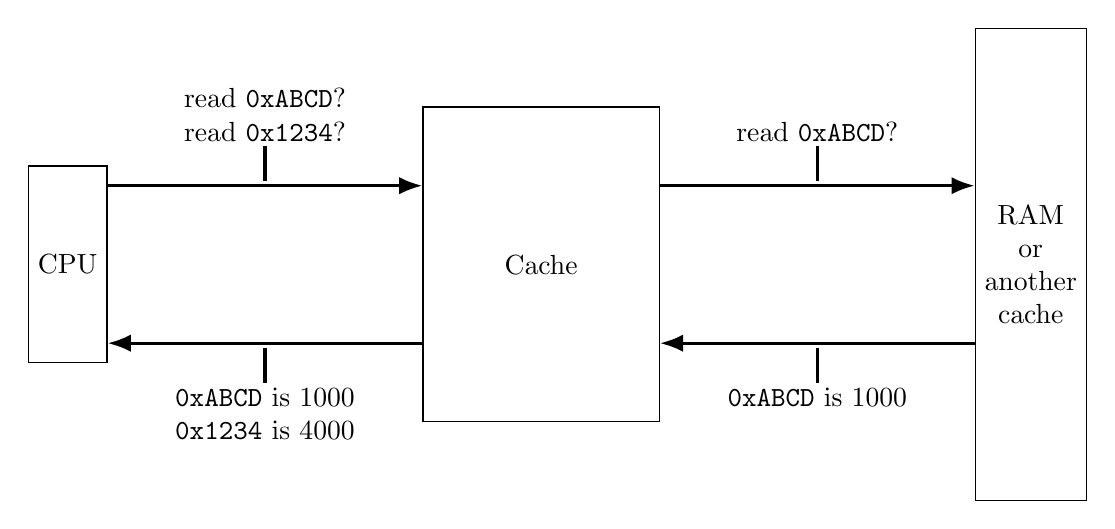
\begin{tikzpicture}
\node[draw,minimum width=1cm,minimum height=2.5cm] (cpu) {CPU};
\node[draw,minimum width=3cm,minimum height=4cm,right=4cm of cpu] (cache) {Cache};
\node[draw,minimum width=1cm,minimum height=6cm,right=4cm of cache,align=center] (mem) {RAM \\ or \\another \\ cache};
\begin{scope}[every node/.style={inner sep=1pt},every pin/.style={align=center,-},every pin edge/.style={-}]
\draw[very thick,-Latex] ([yshift=1cm]cpu.east) -- ([yshift=1cm]cache.west)
    node[midway,pin={north:read {\tt 0xABCD}?\\read {\tt 0x1234}?}] {};
\draw[very thick,Latex-] ([yshift=-1cm]cpu.east) -- ([yshift=-1cm]cache.west)
    node[midway,pin={south:{\tt 0xABCD} is 1000\\{\tt 0x1234} is 4000}] {};
\draw[very thick,-Latex] ([yshift=1cm]cache.east) -- ([yshift=1cm]mem.west)
    node[midway,pin={north:read {\tt 0xABCD}?}] {};
\draw[very thick,Latex-] ([yshift=-1cm]cache.east) -- ([yshift=-1cm]mem.west)
    node[midway,pin={south:{\tt 0xABCD} is 1000}] {};
\end{scope}
% FIXME: hilite hit miss in diagram, seperate into animation
\end{tikzpicture}
\end{frame}

\begin{frame}{memory hierarchy goals}
\begin{itemize}
    \item performance of the fastest (smallest) memory
        \begin{itemize}
            \item hide 100x latency difference? \myemph{99+\% hit (= value found in cache) rate}
        \end{itemize}
    \item capacity of the largest (slowest) memory
\end{itemize}
\end{frame}

